% Code review of RCB
\documentclass[11pt,a4paper]{article}
\usepackage{listings, pdfpages, fullpage}
\title{Ram Control Block Code Review}
\author{Jonathan Ely}

\lstset{language=VHDL,tabsize=2,numbers=left,basicstyle=\small,breaklines=true}

\begin{document}
\maketitle
\section{Introduction}
This report is a code review by Jonathan Ely of the \emph{RCB Block}
which was developed by Farhan Rahman.

\section{Compilation}
Farhan's files compile with no warnings or errors in Modelsim, with
the compilation set to 1993 VHDL and 'Check for Synthesis enabled'.

\section{Synthesis}
Despite Modelsim showing now complaints, Synplify did come up with a 
couple of errors and warnings. 

\subsection{Errors}
The errors all related to the declaration
of the \emph{pix\_write\_cache} instance in \emph{rcb.vhd}. Here, Farhan
forgets to map the \emph{w\_size} and \emph{p\_size} generics causing width
errors since the \emph{w\_size} and \emph{p\_size} generics declared in 
\emph{pix\_write\_cache.vhd} are not the same size as those used in \emph{rcd.vhd}.

\subsection{Warnings}
Synplify displays two warnings from the \emph{rcb.vhd} file.

The first is regarding the OTHERS section of the nextstate CASE statement on line 198.
Synplify states "Others clause is not synthesised", this is because there
are no other states - all the states in the enumerated type have been accounted for.

The last warning is due to an undriven signal in \emph{rcb.vhd}. \emph{delaycmd1}
is not driven at at any point, however it is read from in several IF statements. 
It seems the purpose of this signal is to be able to read the \emph{delaycmd} signal
since VHDL does not allow the reading of an output. To fix this warning line 211 
should be changed to drive \emph{delaycmd1}.

\section{FSMs}
Farhan's FSM appears to work and the selection of states is sensible.

\section{Reset}
All the RCB subentities use the same reset signal that is an input into the rcb entity. The FSM implements a scynchronous reset in the FSM process.

\section{Code Correctness}
\begin{description}
\item[Processes with WAIT FOR:] There are none of these.

\item[Processes with both positive and negative edges:] None.

\item[FOR or WHILE loops with variable length:] There is one FOR loop in 
the \emph{vdin\_compute} process of \emph{pix\_write\_cache}. 
The length of this loop is the range of the \emph{store} array.
The size of the array (16) is declared in \emph{pix\_cache\_pak}.
Although it is not variable sized (the size is set at compile time) it may
be clear to both the user and compiler if a generic was used and included
in the loop declaration.
 
\item[Badly formed processes:] All the sensitivity lists were correct.
There was one signal \emph{delaycmd1} that was not correctly driven
(as discussed earlier in this report)

\item[Signals driven from two different processes:] There are no signals
that are driven in multiple processes.

\end{description}

\section{Design Correctness}
Except the one signal discussed earlier, all signals seem to be 
correctly driven and the specification is adhered to. I don't see any
major problems with this design.

\section{Code Style}
On the whole Farhan's code is fairly clear and well writen. However it would be 
nice if there were more comments.

% Include Farhan's code
\newpage
\appendix
\section{RCB Code}
\subsection{rcb.vhd}
\lstinputlisting{../../src/rcb/rcb.vhd}

\newpage
\subsection{ram\_fsm.vhd}
\lstinputlisting{../../src/ram_fsm/ram_fsm.vhd}

\newpage
\subsection{pix\_word\_cache.vhd}
\lstinputlisting{../../src/pix_word_cache/pix_word_cache.vhd}

\newpage
\subsection{pix\_write\_cache.vhd}
\lstinputlisting{../../src/pix_write_cache/pix_write_cache.vhd}

\newpage
\subsection{pix\_cache\_pak.vhd}
\lstinputlisting{../../src/pix_word_cache/pix_cache_pak.vhd}

%include Farhan's Documentation
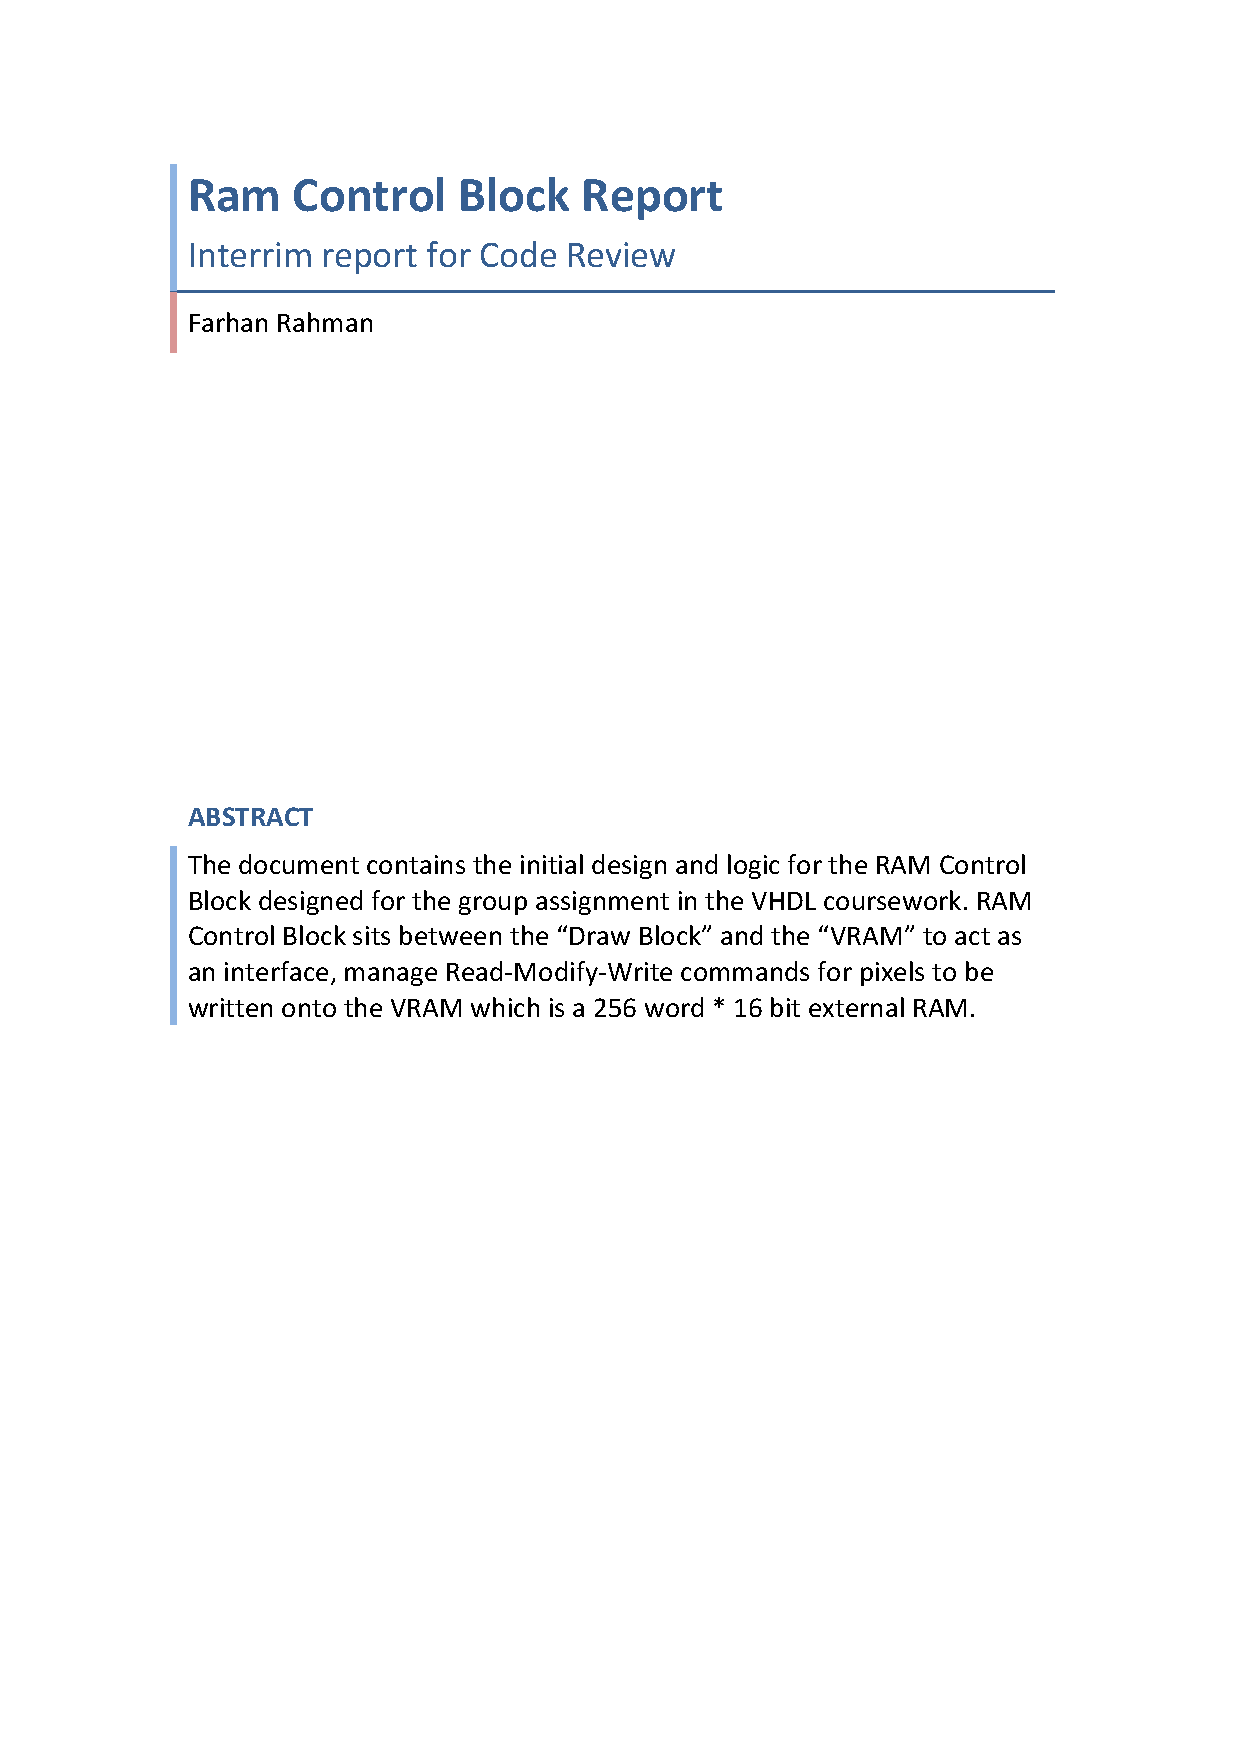
\includepdf[pages=-]{RCBDocumentation.pdf}
\end{document}
